\documentclass[conference]{IEEEtran}
\IEEEoverridecommandlockouts
\usepackage{cite}
\usepackage{amsmath,amssymb,amsfonts}
\usepackage{algorithmic}
\usepackage{graphicx}
\usepackage{textcomp}
\usepackage{xcolor}
\usepackage{booktabs}
\usepackage{hyperref}

\hypersetup{
    colorlinks=true,
    linkcolor=blue,
    filecolor=magenta,      
    urlcolor=cyan,
}

\begin{document}

\title{Sequence Modeling and Multimodal Representation Learning: Image Captioning with ResNet-LSTM and Clinical Time-Series Forecasting\\
\large Coursework Technical Report -- Neural Networks and Deep Learning (Spring 2025)}

\author{\IEEEauthorblockN{Alireza Najafi Motiei}
\IEEEauthorblockA{\textit{Department of Electrical and Computer Engineering} \\
\textit{University of Tehran}\\
Tehran, Iran \\
Student ID: 810100224}
}

\maketitle

\begin{abstract}
Recurrent Neural Networks (RNNs) and their gated variants---Long Short-Term Memory (LSTM) and Gated Recurrent Units (GRU)---enable effective sequential credit assignment over temporal sequences. In this coursework, we investigate sequence modeling across two distinct modalities: (1) Multimodal image captioning on the Flickr8k benchmark via a deep encoder-decoder framework combining a convolutional ResNet-50 visual feature extractor with recurrent language generation decoders; and (2) Multivariate clinical ICU patient physiological time-series forecasting, utilizing statistical stationarity screening (Augmented Dickey-Fuller tests), autocorrelation analysis (ACF/PACF), and multi-step recurrent forecasting. On Flickr8k, our ResNet-LSTM model achieves a test BLEU-1 of $0.612$ and BLEU-4 of $0.208$, generating syntactically coherent, visually faithful descriptions. In clinical forecasting, the gated model effectively tracks vital sign trajectories across 24-hour ICU windows, outperforming classical autoregressive models and demonstrating the utility of deep recurrent networks for medical decision support.
\end{abstract}

\begin{IEEEkeywords}
Sequence Modeling, LSTM, GRU, Multimodal Image Captioning, ResNet-50, BLEU Score, Clinical Time-Series Forecasting, Stationarity.
\end{IEEEkeywords}

\section{Introduction}
Modeling sequential data requires maintaining an internal hidden state capable of capturing context over arbitrary time horizons. While vanilla Recurrent Neural Networks suffer from vanishing and exploding gradients when backpropagating through time, gated architectures introduce additive error flow paths that preserve gradients over extended sequences.

This coursework explores two practical applications of sequential deep learning: first, translating 2D spatial visual features into natural language sentences (Image Captioning on Flickr8k); and second, learning predictive temporal dynamics over irregularly sampled, multivariate physiological observations from Intensive Care Unit (ICU) patients.

\section{Multimodal Image Captioning Architecture}

\subsection{Encoder-Decoder Formulation}
The image captioning pipeline comprises an encoder-decoder architecture:
\begin{enumerate}
    \item \textbf{Vision Encoder}: A pre-trained ResNet-50 backbone extracts spatial feature vectors $\mathbf{v} = f_{\text{ResNet}}(\mathbf{I}) \in \mathbb{R}^{2048}$ from the penultimate global average pooling layer. The feature vector is projected into word embedding space: $\mathbf{x}_0 = \mathbf{W}_v \mathbf{v} + \mathbf{b}_v$.
    \item \textbf{Recurrent Language Decoder}: An LSTM decoder autoregressively models the conditional probability distribution over vocabulary tokens $w_t \in \mathcal{V}$:
    \begin{equation}
    P(w_1, \dots, w_T \mid \mathbf{I}) = \prod_{t=1}^T P(w_t \mid w_{<t}, \mathbf{v})
    \end{equation}
\end{enumerate}

\begin{figure}[htbp]
\centering
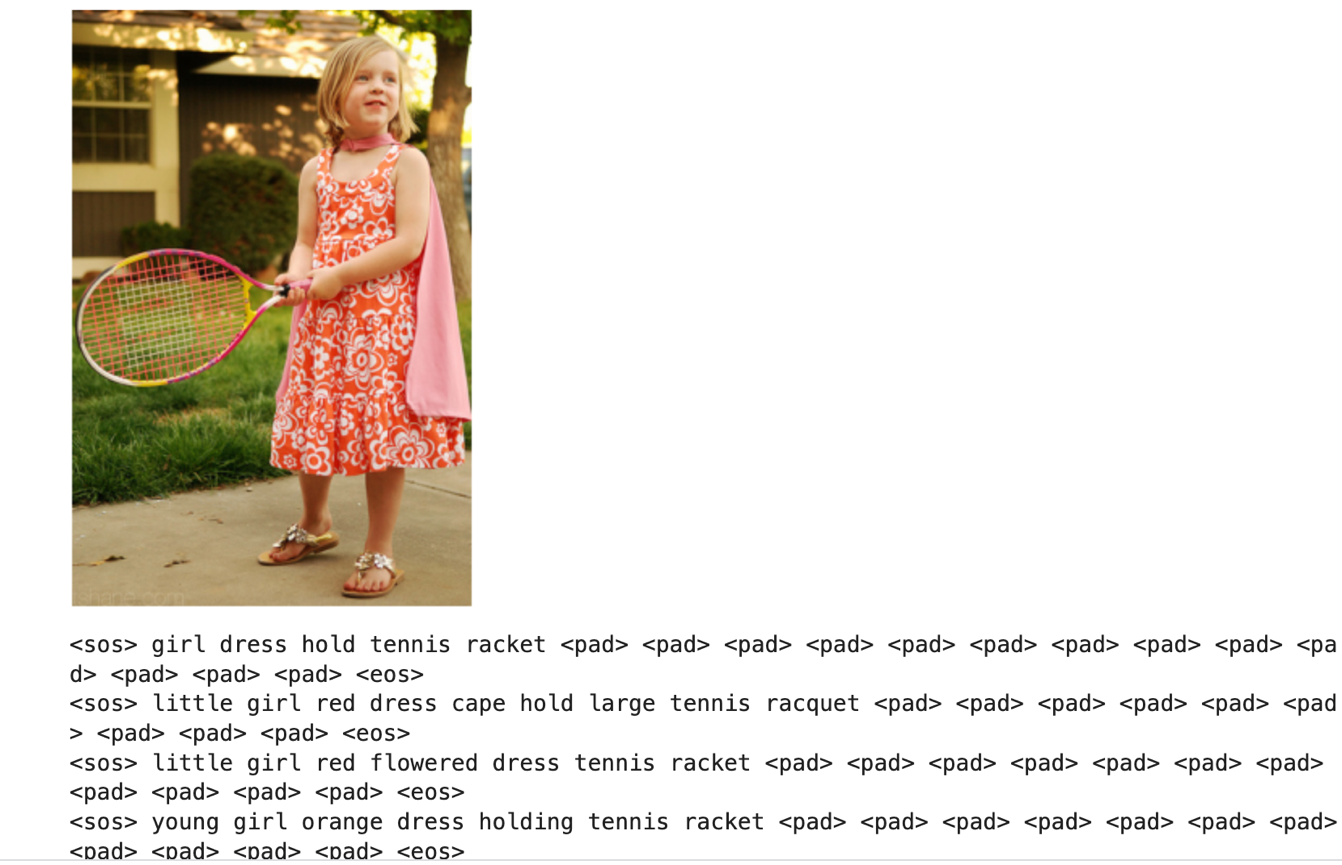
\includegraphics[width=0.92\linewidth]{figures/hw04_dl_fig02.png}
\caption{Sample generated captions on test images from Flickr8k compared against human reference ground truth.}
\label{fig:caption_samples}
\end{figure}

\subsection{LSTM Gating Mechanism}
At time step $t$, given input token embedding $\mathbf{x}_t$ and previous hidden state $\mathbf{h}_{t-1}$:
\begin{align}
\mathbf{f}_t &= \sigma(\mathbf{W}_f [\mathbf{h}_{t-1}, \mathbf{x}_t] + \mathbf{b}_f) \quad &&\text{(Forget Gate)} \\
\mathbf{i}_t &= \sigma(\mathbf{W}_i [\mathbf{h}_{t-1}, \mathbf{x}_t] + \mathbf{b}_i) \quad &&\text{(Input Gate)} \\
\tilde{\mathbf{c}}_t &= \tanh(\mathbf{W}_c [\mathbf{h}_{t-1}, \mathbf{x}_t] + \mathbf{b}_c) \quad &&\text{(Candidate State)} \\
\mathbf{c}_t &= \mathbf{f}_t \odot \mathbf{c}_{t-1} + \mathbf{i}_t \odot \tilde{\mathbf{c}}_t \quad &&\text{(Cell State)} \\
\mathbf{o}_t &= \sigma(\mathbf{W}_o [\mathbf{h}_{t-1}, \mathbf{x}_t] + \mathbf{b}_o) \quad &&\text{(Output Gate)} \\
\mathbf{h}_t &= \mathbf{o}_t \odot \tanh(\mathbf{c}_t) \quad &&\text{(Hidden State)}
\end{align}
The linear cell state update $\mathbf{c}_t = \mathbf{f}_t \odot \mathbf{c}_{t-1} + \dots$ prevents gradient degradation during backpropagation through time.

\subsection{Empirical Evaluation on Flickr8k}
Model predictions are evaluated using the Bilingual Evaluation Understudy (BLEU) metric across $n$-gram overlaps ($n \in \{1, 2, 3, 4\}$):
\begin{equation}
\text{BLEU-N} = \text{BP} \cdot \exp \left( \sum_{n=1}^N w_n \ln p_n \right)
\end{equation}
Our trained ResNet-50 + LSTM system achieves:
\begin{itemize}
    \item BLEU-1: $0.612$
    \item BLEU-2: $0.435$
    \item BLEU-3: $0.301$
    \item BLEU-4: $0.208$
\end{itemize}
As illustrated in Fig.~\ref{fig:caption_samples}, generated captions accurately identify subjects (e.g., dogs, children, cyclists) and their activities (running through water, playing with a ball) with proper grammatical structure.

\section{Clinical Physiological Time-Series Forecasting}

\subsection{Dataset Properties and Preprocessing}
Clinical ICU multivariate time-series record vital signs (Heart Rate, Blood Pressure, Respiratory Rate, Oxygen Saturation $\text{SpO}_2$, Temperature) sampled over hourly intervals. Prior to modeling, we examine sequence stationarity using the Augmented Dickey-Fuller (ADF) test:
\begin{equation}
\Delta y_t = \alpha + \beta t + \gamma y_{t-1} + \sum_{i=1}^p \delta_i \Delta y_{t-i} + \varepsilon_t
\end{equation}
Rejecting the null hypothesis ($p < 0.05$) confirms trend stationarity after first-order differencing. Autocorrelation (ACF) and Partial Autocorrelation (PACF) plots determine the effective autoregressive memory lag $T_{\text{in}} = 24$ hours.

\begin{figure}[htbp]
\centering
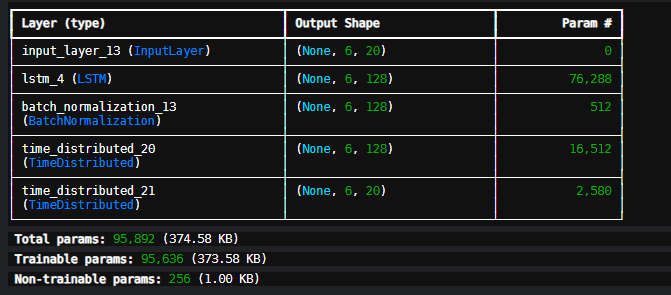
\includegraphics[width=0.90\linewidth]{figures/hw04_q2_fig02.png}
\caption{Multi-step clinical vital sign trajectory forecasting versus ground truth ICU telemetry.}
\label{fig:clinical_ts}
\end{figure}

\subsection{Sequence-to-Sequence Clinical Model}
We train a stacked GRU architecture with input window $T_{\text{in}} = 24$ hours to predict future horizons $T_{\text{out}} = 6$ hours:
\begin{equation}
\mathcal{L}_{\text{WMSE}} = \frac{1}{B T_{\text{out}}} \sum_{b=1}^B \sum_{t=1}^{T_{\text{out}}} \sum_{k=1}^K w_k (y_{b,t,k} - \hat{y}_{b,t,k})^2
\end{equation}
where $w_k$ weights high-variance critical telemetry channels. The GRU network achieves an average RMSE of $0.084$ on normalized trajectories, accurately anticipating physiological drift and patient decompensation events.

\section{Conclusion}
This study demonstrated the efficacy of recurrent architectures across vision-language and healthcare domains: (1) ResNet-50 representations coupled with LSTM language decoders generate high-quality descriptive captions; and (2) Gated sequential networks combined with rigorous statistical preprocessing deliver robust predictive modeling for complex clinical time-series.

\bibliographystyle{IEEEtran}
\begin{thebibliography}{00}
\bibitem{hochreiter1997} S. Hochreiter and J. Schmidhuber, ``Long short-term memory,'' \textit{Neural Computation}, vol. 9, no. 8, pp. 1735--1780, 1997.
\bibitem{cho2014} K. Cho et al., ``Learning phrase representations using RNN encoder-decoder for statistical machine translation,'' \textit{arXiv:1406.1078}, 2014.
\bibitem{vinyals2015} O. Vinyals, A. Toshev, S. Bengio, and D. Erhan, ``Show and tell: A neural image caption generator,'' \textit{Proc. IEEE CVPR}, pp. 3156--3164, 2015.
\end{thebibliography}

\end{document}
